\begin{center}
    \section{Приложение С}\label{appendix:C}
    \textbf{\Large{Раскрытие некоторых математических аспектов квазиклассики на примере задач.}}
\end{center}

\excersize{Упражнение №C1}{darklavender}
\begin{center}
\textit{Пусть частица массой m находится на n-ом уровне гармонического осциллятора. Найдите точку поворота $x_2$. Насколько далеко от точки поворота может улететь частица перед тем как ошибка из-за линеаризации потенциала достигнет 1\%?}.\\
\textit{При $z\geq 5$ применение асимптотики для функции Эйри $Ai(z)$ даёт ошибку в 1\%. Для расстояния вылета за точку поворота d найти наименьший уровень n, при котором $\alpha d\geq 5$}.
\end{center}
Напомню, как выглядит энергия для квантового гармонического осциллятора: 
\[E_n = \hbar\omega(n + 1/2).\] Точку поворота можно найти из условия p = 0:
\begin{gather*} 
p(x_2) = \sqrt{2mE_n - m^2\omega^2x_2^2} = 0\; => \; 2mE_n = m^2\omega^2x_2^2 \; => \\
=>\; x_2 = \sqrt{\frac{(2n + 1)\hbar}{m\omega}}
\end{gather*}
Пусть d -- искомое расстояние, на которое может улететь частица при сохранении ошибки в 1\%. Тогда найдём d из следующей формулы:
\[
\frac{V(x_2 + d) - V_{lin}(x_2 + d)}{V(x_2)} = 0.01
\]
Найдём $V_{lin}(x_2 + d)$:
\begin{gather*}
V_{lin}(x) = V(x_2) + V'(x_2)(x - x_2) = \frac{m\omega^2 x_2^2}{2} + (m\omega^2 x_2)(x-x_2)\; => \;\\
V_{lin}(x_2 + d) = \frac{m\omega^2 x_2^2}{2} + m\omega^2 x_2d.
\end{gather*}
Подставив это в формулу, получим:
\begin{gather*}
    \frac{V(x_2 + d) - V_{lin}(x_2 + d)}{V(x_2)} = \frac{\frac{m\omega^2 (x_2 + d)^2}{2} - \frac{m\omega^2 x_2^2}{2} - m\omega^2 x_2d.}{\frac{m\omega^2 x^2}{2}} = \\
    = \left(\frac{d}{x_2}\right)^2 =  0.01\; => \; d = 0.1x_2.
\end{gather*}

Найдём уровень энергии, при котором выполняется $\alpha d \geq 5$. Для этого вспомним, что $\alpha = (2m^2\omega^2x_2/\hbar)^{1/3}$. Тогда, пользуясь полученным выше соотношением:
\begin{gather*}
    0.1x_2\left[\frac{2m^2\omega^2x_2}{\hbar^2}\right]^{1/3} \geq 5\; => \; \frac{2m^2\omega^2 x_2^4}{\hbar^2} \geq 50^3 \; => \\
    => \; \frac{2m^2\omega^2}{\hbar^2} \frac{(2n + 1)^2\hbar^2}{m^2\omega^2} \geq 50^3 \; => \; (2n+1)^2 \geq 50^2 \cdot 25 \; => \; n \geq 124.5
\end{gather*}
Получается, что при значениях $n\geq 125$ линейная аппроксимация и асимптотика функции Эйри не будут превышать ошибку в 1\%. В квазиклассических системах n обычно сильно больше.
\csquare{darklavender}

\excersize{Упражнение №C2}{darklavender}
\begin{center}
\textit{Выведите формулы связи для убывающего потенциала (рисунок \ref{fig C.1})}.
\end{center}
\begin{figure}[ht]
\centering
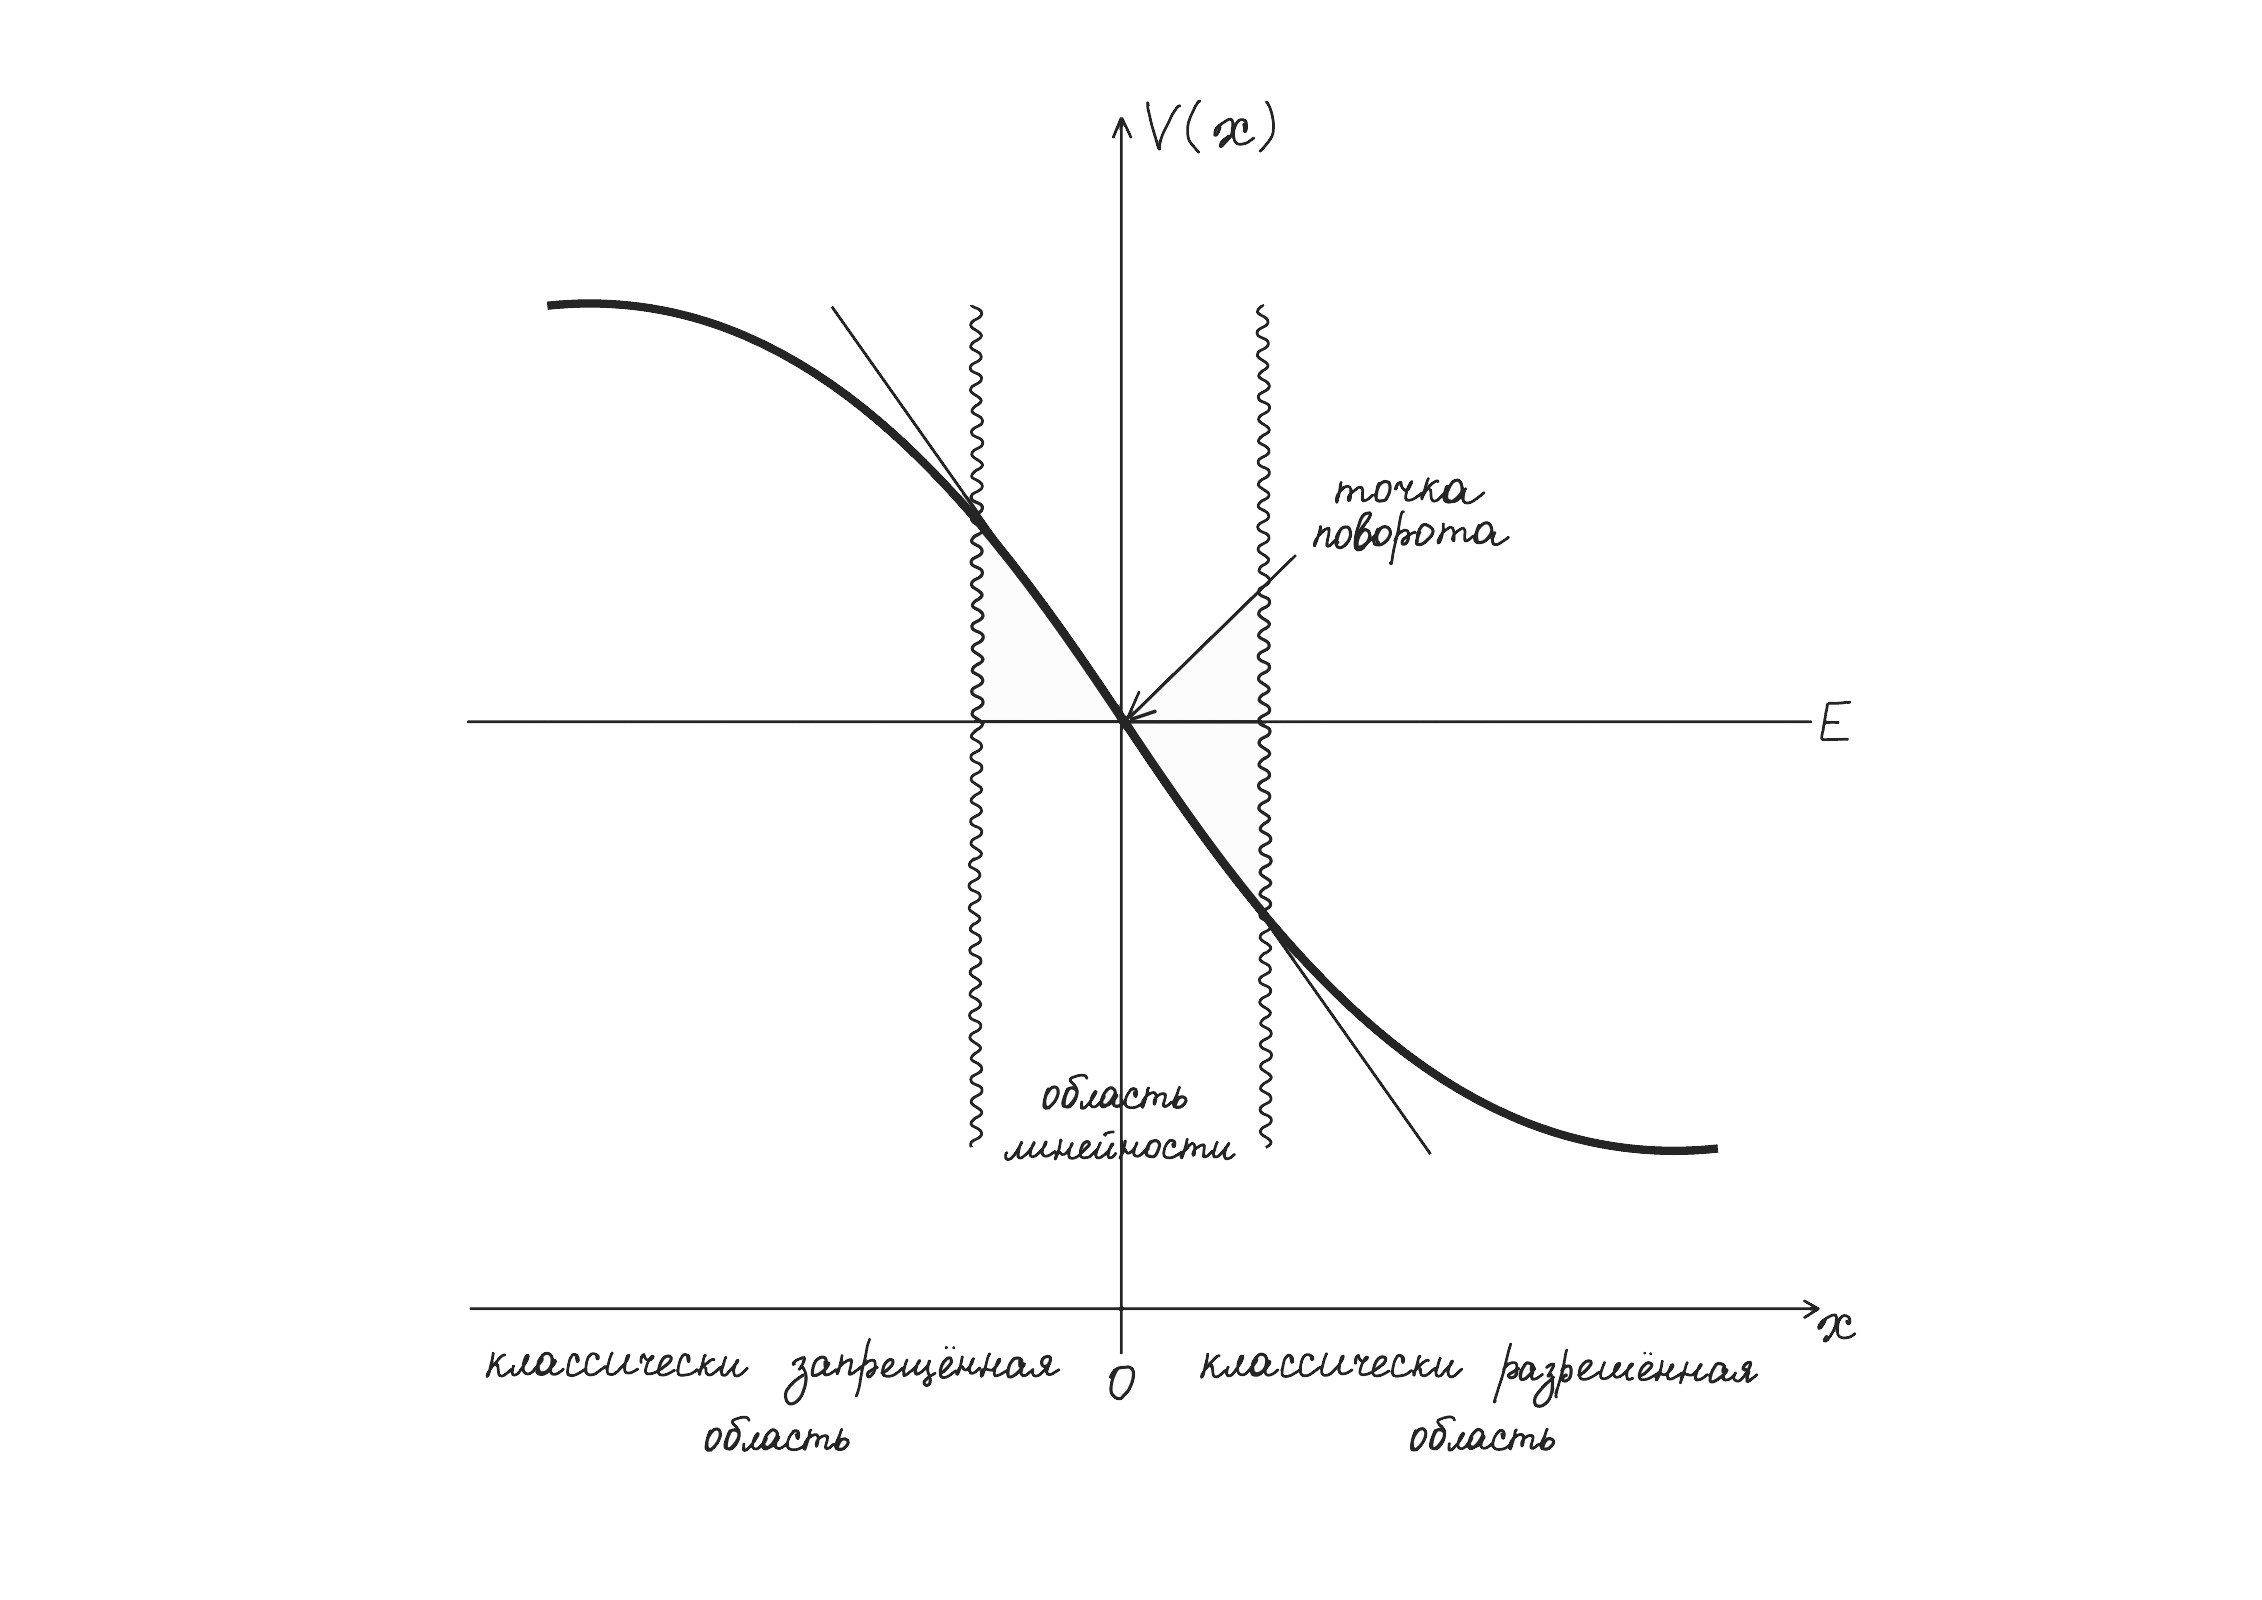
\includegraphics[scale=0.21]{appendix/images/left-turning-point.jpg}
\caption{Потенциальный барьер}
\label{fig C.1}
\end{figure}
Подход будет аналогичным, как и для правой точки. Для начала запишем волновую функцию, коэффициенты которой будем искать:
\[
\psi(x) \simeq 
\begin{cases}
     \frac{1}{\sqrt{|p|}}\left[ Ae^{-\frac{1}{\hbar}\int\limits_x^{0} |p| dx'} \right],\; x < 0;\\
    \frac{1}{\sqrt{p}}\left[ Be^{\frac{i}{\hbar}\int\limits_{0}^{x} p dx'} + Ce^{-\frac{i}{\hbar}\int\limits_{0}^{x} p dx'} \right],\; 0 < x.
\end{cases}
\]
Запишем линеаризованный потенциал (обращаю внимание на то, что в этот раз первая производная будет отрицательной, так как потенциал убывает) как $V(x) \approx E + V'(0)x$. Тогда уравнение Шрёдингера будет иметь следующий вид:
\[
    \frac{d^2\psi_T}{d\psi_T^2} = -\alpha^3 x\psi_p, \quad \alpha = \left( \frac{2m|V'(0)|}{\hbar^2} \right)^{1/3}
\]
Решением этого дифференциального уравнения опять будут функции Эйри:
\[
\psi_T(x) = aAi(-\alpha x) + bBi(-\alpha x)
\]
Посчитаем импульс:
\[
p \simeq \sqrt{2m|V'(0)|x} = \hbar\alpha^{3/2}\sqrt{x}
\]
Подставим импульс в интеграл для классически запрещённой области:
\[
\int\limits_{x}^{0} |p| dx' = \hbar\alpha^{3/2} \int\limits_{x}^{0}\sqrt{-x'} dx' = \frac{2}{3}\hbar(-\alpha x)^{3/2}
\]
Запишем волновую функцию в той же области с полученным значением интеграла:
\[
\psi(x) \simeq \frac{A}{\hbar^{1/2}\alpha^{3/4}(-x)^{1/4}} e^{-\frac{2}{3}(-\alpha x)^{3/2}}
\]
Воспользуемся аппроксимацией для больших значений $-\alpha x \gg 0$:
\[
\psi_T \approx \frac{a}{2\pi^{1/2}(-\alpha x)^{1/4}}e^{-\frac{2}{3}(-\alpha x)^{3/2}} + \frac{b}{\pi^{1/2}(-\alpha x)^{1/4}}e^{\frac{2}{3}(-\alpha x)^{3/2}}
\]
Сравнивая две функции, получим:
\[
a = 2A\sqrt{\frac{\pi}{\alpha\hbar}},\; b = 0
\]

Проделаем аналогичные рассуждения для классически разрешенной области:
\begin{gather*}
\int\limits_{0}^{x} p dx' = \hbar\alpha^{3/2} \int\limits_{0}^{x}\sqrt{x'} dx' = \frac{2}{3}\hbar(\alpha x)^{3/2}\; =>\\
=>\; \psi(x) \simeq \frac{1}{\hbar^{1/2}\alpha^{3/4}x^{1/4}}\left[ Be^{i\frac{2}{3}(\alpha x)^{3/2}} + Ce^{-i\frac{2}{3}(\alpha x)^{3/2}} \right]
\end{gather*}
В этот раз воспользуемся аппроксимацией для малых значений $\alpha x \ll 0$:
\[
\psi_T \approx \frac{a}{\pi^{1/2}(\alpha x)^{1/4}}\sin\left[\frac{2}{3}(\alpha x)^{3/2} + \frac{\pi}{4}\right] = \frac{a}{\pi^{1/2}(\alpha x)^{1/4}}\frac{1}{2i}\left[ e^{i\frac{\pi}{4}}e^{i\frac{2}{3}(\alpha x)^{3/2}} - e^{-i\frac{\pi}{4}}e^{-i\frac{2}{3}(\alpha x)^{3/2}} \right].
\]
Опять сравнив две волновые функции, получим:
\[
B = \frac{a}{2i}\sqrt{\frac{\alpha\hbar}{\pi}}e^{i\frac{\pi}{4}},\; C = -\frac{a}{2i}\sqrt{\frac{\alpha\hbar}{\pi}}e^{-i\frac{\pi}{4}}
\]
Подставим ранее полученную a, выраженную через коэффициент A:
\[
B = -ie^{i\frac{\pi}{4}}A,\; C = ie^{-i\frac{\pi}{4}}A
\]
Подставляя эти значения в первоначальную функцию для x>0, получим:
\[
\psi(x) \simeq \frac{-iA}{\sqrt{p}}\left[ e^{\frac{i}{\hbar}\int\limits_{0}^{x} p dx' + i\frac{\pi}{4}} - e^{-\frac{i}{\hbar}\int\limits_{0}^{x} p dx' - i\frac{\pi}{4}} \right] = \frac{2A}{\sqrt{p}}\sin\left[ \frac{1}{\hbar} \int\limits_0^{x}p dx' + \frac{\pi}{4} \right]
\]
Запишем итоговый вид волновой функции для левой точки поворота:
\[
\psi_L(x) \simeq 
\begin{cases}
    \frac{A}{\sqrt{|p|}}e^{-\frac{1}{\hbar} \int\limits_{x}^{x_1} |p|\,dx'},\; \text{при } x < x_1\\
    \frac{2A}{\sqrt{p}}\sin\left[ \frac{1}{\hbar} \int\limits_{x_1}^{x} p\,dx' + \frac{\pi}{4} \right], \; \text{при } x > x_1\\
\end{cases}
\]
\csquare{darklavender}
\newpage
\excersize{Упражнение №C3}{darklavender}
\begin{center}
\textit{Рассмотрите задачу с потенциальным барьером (рисунок \ref{fig C.2}). Найдите волновую функцию. Запишите, какой в этом случае будет коэффициент прохождения $T$}.
\end{center}

\begin{figure}[h!]
\centering
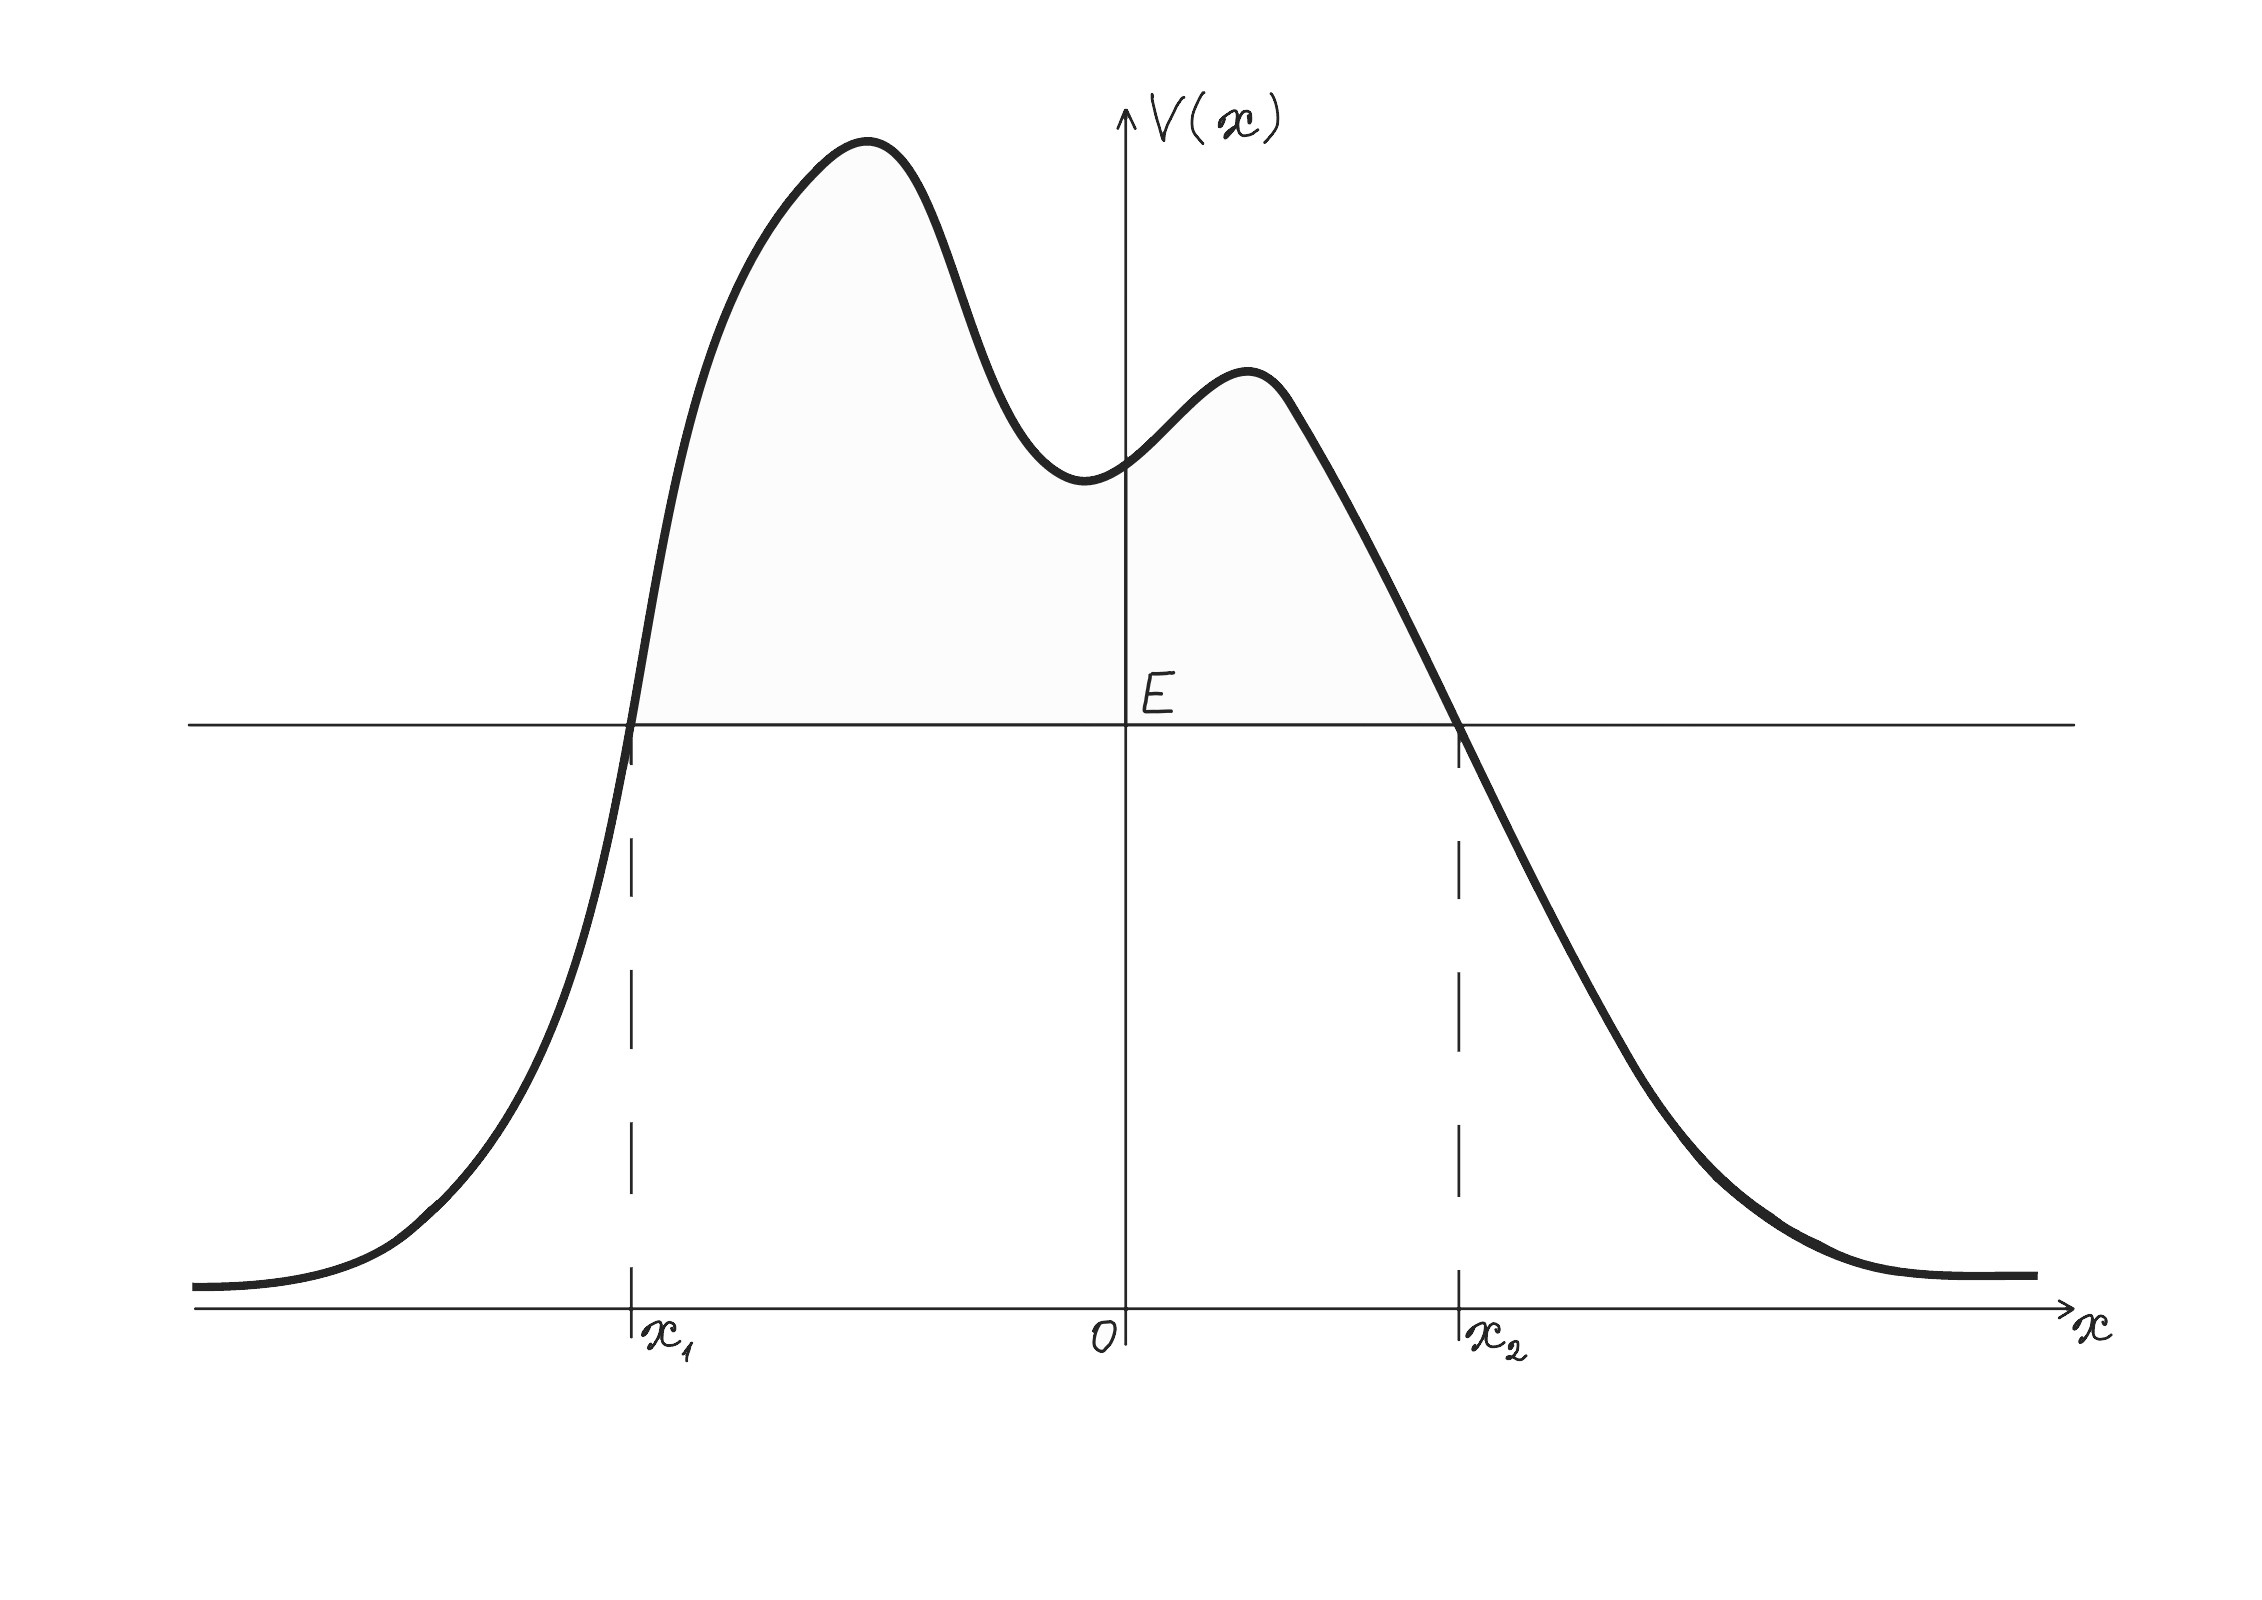
\includegraphics[scale=0.16]{appendix/images/barier.jpg}
\caption{Потенциальный барьер}
\label{fig C.2}
\end{figure}

Запишем общую волновую функцию:
\[
\psi(x) \simeq 
\begin{cases}
    \frac{1}{\sqrt{p}}\left[ Ae^{\frac{i}{\hbar}\int\limits_x^{x_1} p dx'} + Be^{-\frac{i}{\hbar}\int\limits_x^{x_1} p dx'} \right],\; x<x_1;\\
    \frac{1}{\sqrt{|p|}}\left[ Ce^{\frac{1}{\hbar}\int\limits_{x_1}^{x} |p| dx'} + De^{-\frac{1}{\hbar}\int\limits_{x_1}^{x} |p| dx'} \right],\; x_1< x < x_2;\\
    \frac{1}{\sqrt{p}}\left[ Fe^{\frac{i}{\hbar}\int\limits_{x_2}^{x} p dx'}\right],\; x > x_2.
\end{cases}
\]
Внутри барьера запрещённая область, поэтому импульс стоит под модулем. Слева приходит обычная волна и улетает отражённая, поэтому экспоненты две. Справа же только волна, которая прошла сквозь барьер, поэтому слагаемое только одно. 

Для нахождения коэффициентов будем использовать тот же подход, что мы использовали в нахождении волновых функций для точек поворота в потенциальной яме. Тем более, что при аппроксимации функций Эйри получатся те же самые $\psi_T$. Итак, считаем интеграл от импульса, подставляем в волновую функцию для правой области левой точки поворота ($x_1 < x < x_2$), получим:
\[
    \psi(x) \simeq \frac{1}{\hbar^{1/2}\alpha^{3/4}x^{1/4}}\left[ Ce^{\frac{2}{3}(\alpha x)^{3/2}} + De^{-\frac{2}{3}(\alpha x)^{3/2}} \right]
\]
Аппроксимация остаётся такой же:
\[
    \psi_T \approx \frac{a}{2\pi^{1/2}(\alpha x)^{1/4}}e^{-\frac{2}{3}(\alpha x)^{3/2}} + \frac{b}{\pi^{1/2}(-\alpha x)^{1/4}}e^{\frac{2}{3}(-\alpha x)^{3/2}}
\]
Сравнивая, получим:
\[
a = 2D\sqrt{\frac{\pi}{\alpha\hbar}},\; b = C\sqrt{\frac{\pi}{\alpha\hbar}}
\]
Для левой области получим следующие волновые функции:
\begin{align*}
    \psi(x) &\simeq \frac{1}{\hbar^{1/2}\alpha^{3/4}(-x)^{1/4}}\left[ Ae^{i\frac{2}{3}(\alpha x)^{3/2}} + Be^{-i\frac{2}{3}(\alpha x)^{3/2}} \right];\\
    \psi_T(x) &\approx \frac{a}{\pi^{1/2}(\alpha x)^{1/4}}\sin\left[\frac{2}{3}(\alpha x)^{3/2} + \frac{\pi}{4}\right] + \frac{b}{\pi^{1/2}(\alpha x)^{1/4}}\cos\left[\frac{2}{3}(\alpha x)^{3/2} + \frac{\pi}{4}\right] = \\ 
    & = \frac{a}{2\pi^{1/2}(-\alpha x)^{1/4}}\left[ (-ia + b)e^{i\frac{\pi}{4}}e^{i\frac{2}{3}(\alpha x)^{3/2}} + (ia+b)e^{-i\frac{\pi}{4}}e^{-i\frac{2}{3}(\alpha x)^{3/2}} \right].
\end{align*}
Вновь сравнивая, получим:
\[
A = \sqrt{\frac{\hbar\alpha}{\pi}}\left( \frac{-ia + b}{2} \right)e^{i\frac{\pi}{4}},\; B = \sqrt{\frac{\hbar\alpha}{\pi}}\left( \frac{ia + b}{2} \right)e^{-i\frac{\pi}{4}}
\]
Подставим ранее полученные значения коэффициентов a и b:
\[
    A = \left( \frac{C}{2} - iD \right)e^{i\frac{\pi}{4}}, \; B = \left( \frac{C}{2} + iD \right)e^{-i\frac{\pi}{4}}
\]

Для правой точки поворота, для начала, перепишем волновую функцию для запрещённой области в следующем виде:
\[
\psi(x) \simeq \frac{1}{\sqrt{|p|}} \left[ Ce^{\frac{1}{\hbar}\int\limits_{x_1}^{x_2} |p| dx + \frac{1}{\hbar}\int\limits_{x_2}^{x} |p| dx'} + De^{-\frac{1}{\hbar}\int\limits_{x_1}^{x_2} |p| dx - \frac{1}{\hbar}\int\limits_{x_2}^{x} |p| dx'} \right]
\]

Введём новые обозначения. Пусть $\gamma = \frac{1}{\hbar}\int\limits_{x_1}^{x_2} |p| dx$, $C' = De^{-\gamma}$ и $D' = Ce^{\gamma}$ и сместим ноль в правую точку поворота. Тогда волновая функция будет иметь следующий вид:
\[
   \psi(x) \simeq 
   \begin{cases}
   \frac{1}{\sqrt{|p|}}\left[ C'e^{\frac{1}{\hbar}\int\limits_{x}^{0} |p| dx'} + D'e^{-\frac{1}{\hbar}\int\limits_{x}^{0} |p| dx'} \right],\; x < 0;\\
   \frac{1}{\sqrt{p}}\left[ Fe^{\frac{i}{\hbar}\int\limits_{0}^{x} p dx'} \right],\; x > 0
   \end{cases}
\]
Далее делаем всё по аналогии:
\[
\begin{cases}
    \psi(x) \simeq \frac{1}{\hbar^{1/2}\alpha^{3/4}(-x)^{1/4}}\left[ C'e^{\frac{2}{3}(\alpha x)^{3/2}} + D'e^{-\frac{2}{3}(\alpha x)^{3/2}} \right]\\
    \psi_T \approx \frac{a}{2\pi^{1/2}(-\alpha x)^{1/4}}e^{-\frac{2}{3}(-\alpha x)^{3/2}} + \frac{b}{\pi^{1/2}(-\alpha x)^{1/4}}e^{\frac{2}{3}(-\alpha x)^{3/2}}
\end{cases}
 \; => \;
 \begin{cases}
     a = 2\sqrt{\frac{\pi}{\hbar\alpha}}D'\\
     b = \sqrt{\frac{\pi}{\hbar\alpha}}C'
 \end{cases}
\]
Рассмотрим классически разрешённую область:
\[
\begin{cases}
    \psi(x) \simeq \frac{1}{\hbar^{1/2}\alpha^{3/4}x^{1/4}}Fe^{i\frac{2}{3}(\alpha x)^{3/2}}\\
    \psi_T \approx \frac{a}{2\pi^{1/2}(\alpha x)^{1/4}}\left[ (-ia + b)e^{i\frac{\pi}{4}}e^{i\frac{2}{3}(\alpha x)^{3/2}} + (ia+b)e^{-i\frac{\pi}{4}}e^{-i\frac{2}{3}(\alpha x)^{3/2}} \right]
\end{cases}
 \; => \; (ia + b) = 0.
\]
Тогда, выразим коэффициенты $a$ и $b$ через $F$:
\[
F = \sqrt{\frac{\hbar\alpha}{\pi}}\left( \frac{-ia + b}{2} \right)e^{i\frac{\pi}{4}}\; => \; b = \sqrt{\frac{\pi}{\hbar\alpha}} e^{-i\frac{\pi}{4}}F, \; a = i\sqrt{\frac{\pi}{\hbar\alpha}} e^{-i\frac{\pi}{4}}F
\]
Найдём связь коэффициентов $C$ и $D$ с коэффициентом $F$:
\[
\begin{cases}
    C' = e^{-i\frac{\pi}{4}}F\\
    D' = \frac{i}{2}e^{-i\frac{\pi}{4}}F
\end{cases}
\; => \;
\begin{cases}
    D = e^{-i\frac{\pi}{4}}Fe^{\gamma}\\
    C = \frac{i}{2}e^{-i\frac{\pi}{4}}Fe^{-\gamma}
\end{cases}
\]
Подставив их в формулу для $A$, получим нужную нам связь между $A$ и $F$:
\[
A = \left( \frac{C}{2} - iD \right)e^{i\frac{\pi}{4}} = i\left( \frac{e^{-\gamma}}{4} - e^{\gamma} \right)F
\]
Коэффициент прохождения есть отношение коэффициента прошедшей к коэффициенту падающей волны $T \frac{|F|^2}{|A|^2}$. Найдём его в нашей задаче:
\[
T = \frac{1}{(e^{\gamma} - e^{-\gamma}/4)^2} = \frac{e^{-2\gamma}}{[1-(e^{-\frac{\gamma}{2}})^2]^2}
\]
При $\gamma \gg 1$ знаменатель близок к 1 и тогда можно записать коэффициент пропускания как
\[
T = e^{-2\gamma}
\]
\csquare{darklavender}

\excersize{Упражнение №C4}{darklavender}
\begin{center}
\textit{Частица массой m с энергией E ``заперта'' в области $r<r_1$, где $U(r) = -U_0$. При $r > r_1$ потенциал имеет вид:}
\[
U(r) = \frac{2Ze^2}{r}; \; E \ll \frac{2Ze^2}{r_1}
\]
\textit{Воспользовавшись квазиклассическим приближением, найдите коэффициент прохождения сквозь барьер.}
\end{center}

\begin{figure}[h!]
\centering
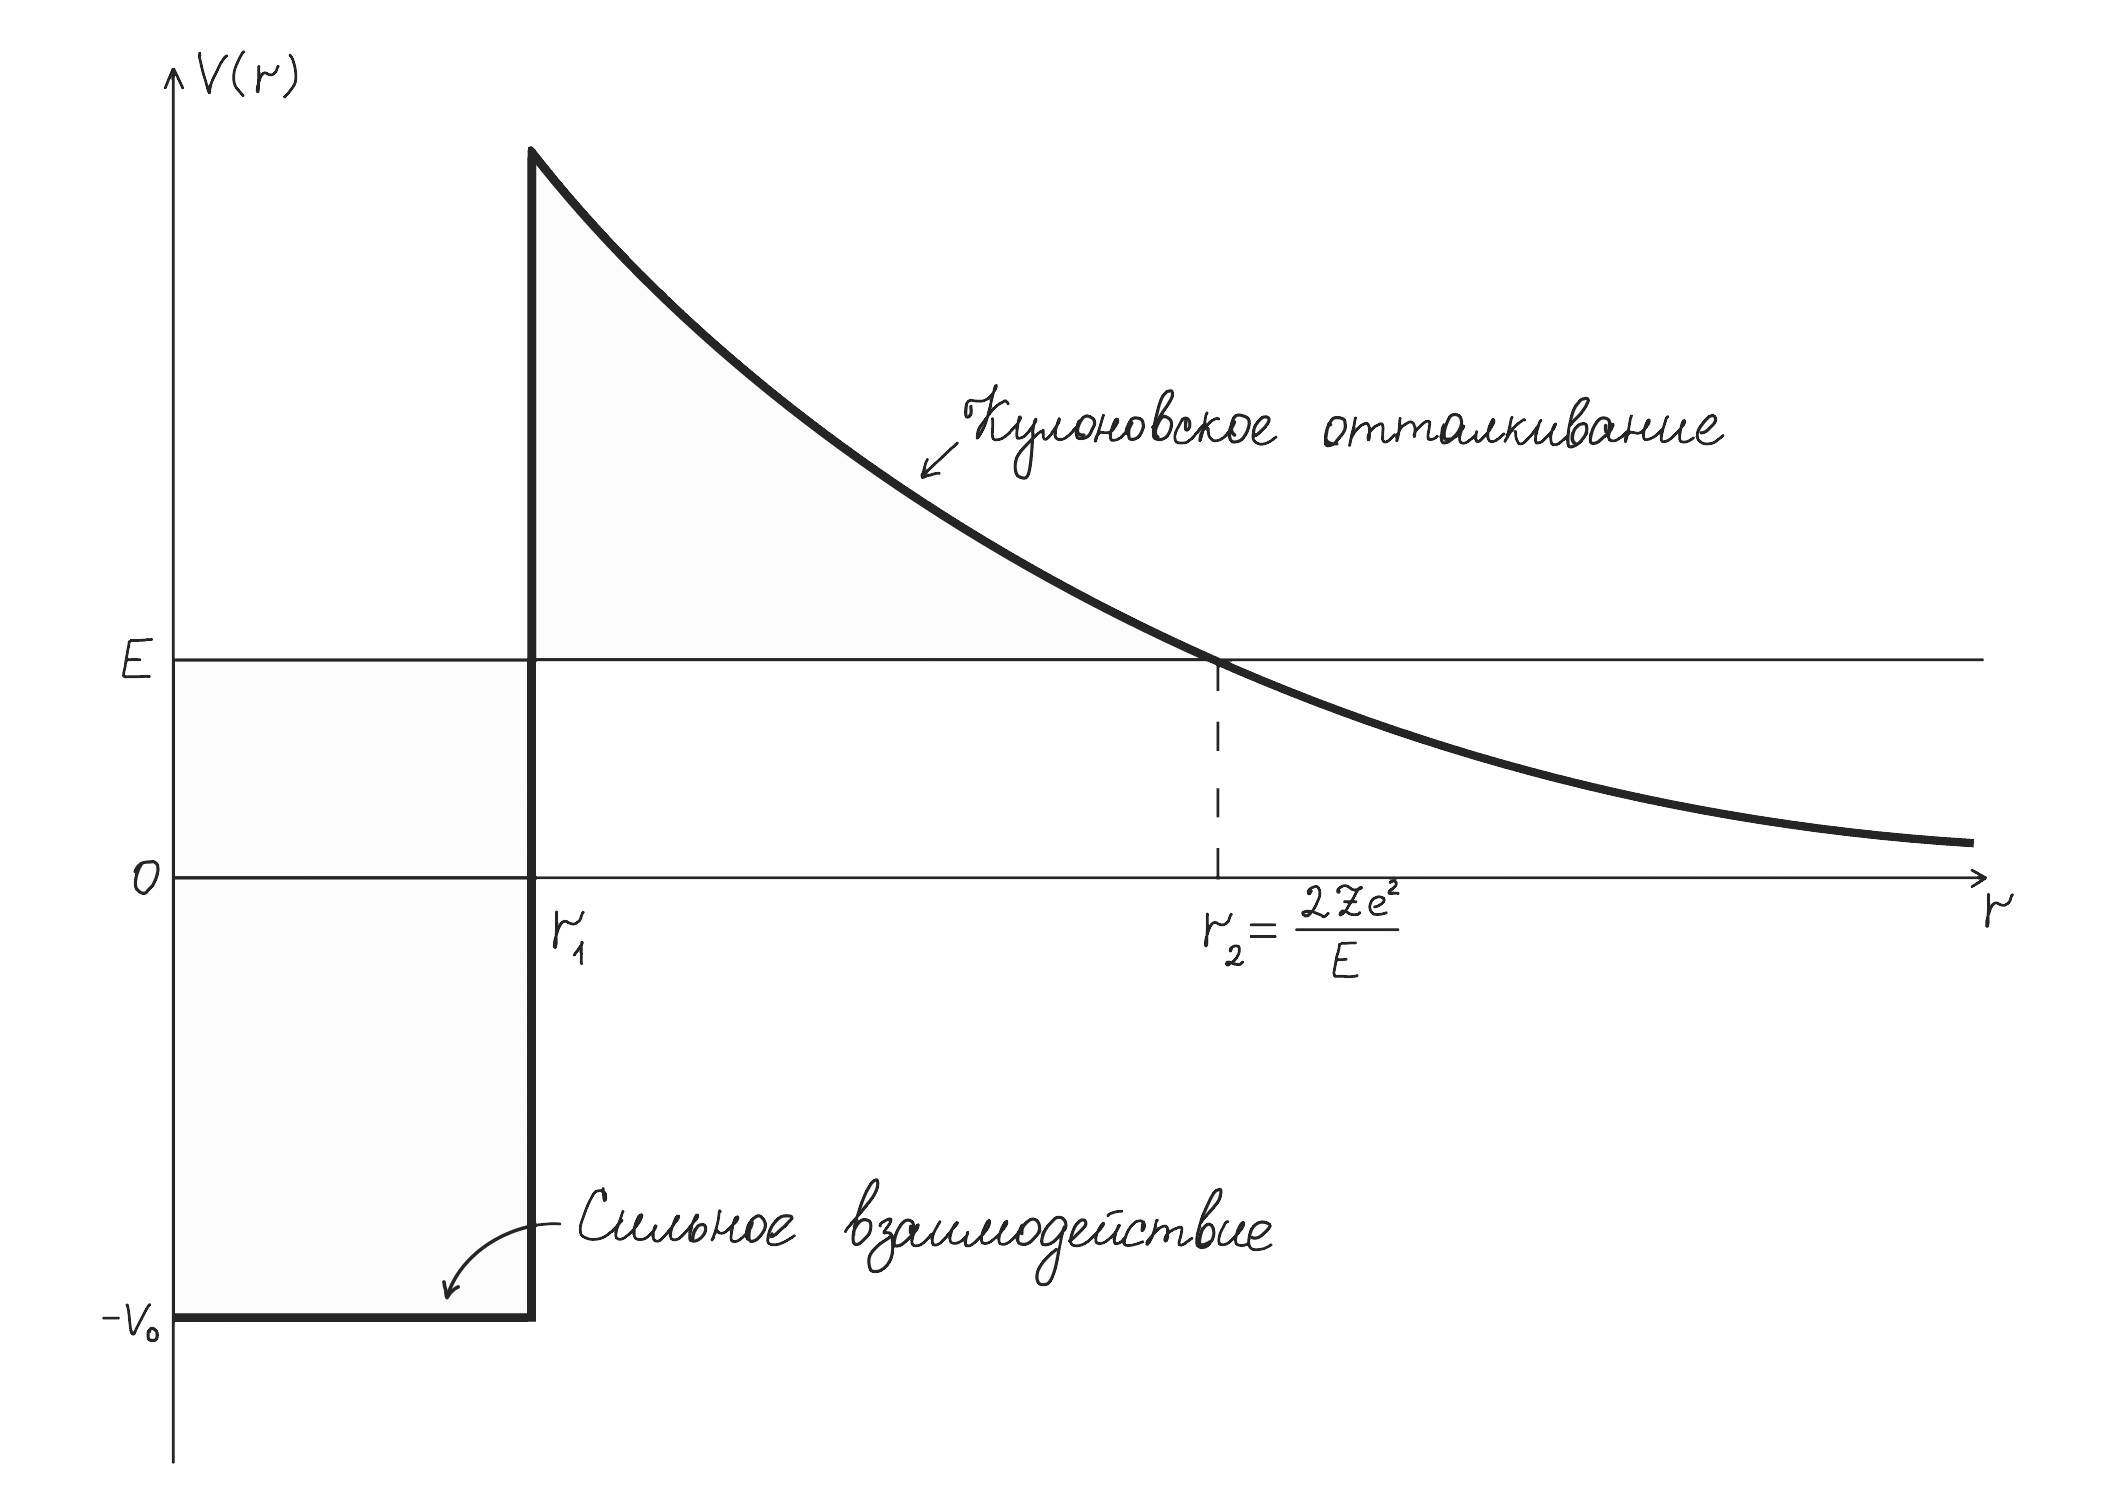
\includegraphics[scale=0.2]{appendix/images/alpha-decay.jpg}
\caption{Модель альфа излучения}
\label{fig C.3}
\end{figure}

Из предыдущей задачи мы знаем, что коэффициент прохождения можно выразить как $T = e^{-2\gamma}$, где $\gamma = \int_{x_1}^{x_2}p dx$. Определим правую точку поворота как $r_2 = 2Ze^2/E$. Посчитаем гамму для нашей задачи:
\begin{align*}
    \gamma & = \frac{1}{\hbar}\int\limits_{r_1}^{r_2}\sqrt{\frac{2Ze^2}{r} - E}dx = \frac{\sqrt{2mE}}{\hbar} \int\limits_{r_1}^{r_2} \sqrt{\frac{r_2}{r} - 1}dx = \\
    &= (r = r_2\sin^2 u) = \frac{\sqrt{2mE}}{\hbar}\left[ r_2\left( \frac{\pi}{2} - \arcsin\sqrt{\frac{r_1}{r_2}} \right) - \sqrt{r_1 (r_2 - r_1)}\right]
\end{align*}
На практике оказывается, что $r_1 \ll r_2$. Тогда $\arcsin (x)\approx x$ и гамма равна
\[
\gamma \simeq \frac{\sqrt{2mE}}{\hbar}\left[ \frac{\pi}{2}r_2 - 2\sqrt{r_1 r_2} \right] = K_1\frac{Z}{\sqrt{E}} - K_2\sqrt{Zr_1},
\]
где $K_1 = \frac{e^2\pi\sqrt{2m}}{\hbar}$ и $K_2 = \frac{4e\sqrt{m}}{\hbar}$. Тогда коэффициент прохождения равен
\[
T = e^{-2\gamma} = e^{2K_2\sqrt{Zr_1} - K_1\frac{2Z}{\sqrt{E}}}
\]
\csquare{darklavender}